\documentclass{article}
\usepackage[utf8]{inputenc}

\usepackage[T2A]{fontenc}
\usepackage[utf8]{inputenc}
\usepackage[polutonikogreek, english,russian]{babel}
\usepackage{csquotes}

\usepackage{hyperref}
\hypersetup{
    colorlinks, citecolor=black, filecolor=black, linkcolor=black, urlcolor=black
}

\usepackage{graphicx}
\graphicspath{ {./images/} }

\newtheorem{definition}{Определение}

\title{Философия}
\author{Лисид Лаконский}
\date{December 2022}

\begin{document}

\maketitle
\tableofcontents
\pagebreak

\section{Философия - 08.12.2022}

\subsection{Онтология}

\begin{flushleft}

\begin{definition}
Онтология (новолат. ontologia от др.-греч. \textgreek{ὄν}, род. п. \textgreek{ὄντος} — сущее, то, что существует + \textgreek{λόγος} — учение, наука) — учение о бытии.
\end{definition}

\begin{definition}
Онтология — совокупность некоторых общих допущений (эмпирические не верифицируемых) о характере мира.
\end{definition}

Пример онтологических допущений: мир бесконечен в пространстве (мир конечен в пространстве), мир имеет конец во времени (не имеет конца во времени)

Пример современной онтологии: мир имел начало во времени, бесконечен в пространстве, имеет конец во времени, упорядочен (существует причинность и так далее) — физика.

\subsection{Категории бытия}

\subsubsection{Бытие}

Как определять бытие не надо:

\begin{enumerate}
    \item Бытие — это всё
    \item Бытие — это способность к существованию
\end{enumerate}

Более вменяемое определение: \textbf{бытие} — понятие самой высокой степени абстракции; понятие всех понятий; понятие, которое включает в себя все остальные понятия

\subsubsection{Существование}

Почему вообще в мире что-то есть? Наиболее удачное определение:

С точки зрения логики, \textbf{существовать} — значит быть значением квантифицированной переменной; то есть, значением переменной, к которой был приписан квантор существования.

Две \textbf{формы бытия}:

\begin{enumerate}
    \item Материальное — можно эмпирически верифицировать.
    \item Идеальное — обладают объекты духовной культуры.
\end{enumerate}

Иначе выделяют две формы бытия: \textbf{социальное} и \textbf{человеческое} (не рекомендуется говорить об этом на экзамене, лучше скажите про материальное и идеальное).

Человеческое бытие — \textbf{экзистенция}, иногда выделяют как отдельную форму бытия.

\subsection{Онтология диалектического материализма}

Исток диалектического материализма (далее — диамат) — \textbf{середина девятнадцатого века}

\begin{definition}
    Материя — объективная действительность (то, что существует независимо от нашего сознания); центральная категория диалектического материализма
\end{definition}

Согласно диамату, \textbf{сознание — тоже материя}, так как имеет материальный субстрат — мозг. Понимание материи в диамате \textbf{отличается} от понимания материи в современной философии и современной науке (до какой степени материальна энергия [поле] в физике)

\subsubsection{Аттрибуты материи}

\begin{enumerate}
    \item \textbf{Движение} — \textbf{всякое изменение} (становление, как это называли древние греки); возможно благодаря тому, что в мире существует множество объектов; имманентный аттрибут - присущий самой материи. Пять форм движения материи (в иерархическом порядке, от низшего к высшему):
    \begin{enumerate}
        \item \textbf{механическая} — перемещение объекта в пространстве
        \item \textbf{физическая} — уровень физического взаимодействия; уровень влияния всяких физических взаимодействий: инерции, силы трения, всяких других сил и так далее
        \item \textbf{химическая} — конкретное взаимодействие веществ
        \item \textbf{биологическая} — движение живой материи (материи в живых существах); все процессы в живых существах
        \item \textbf{социальная}; общество — чисто материальный субстрат, так как общество невозможно без людей — материальных сущностей; общественные процессы протекают независимо от нашего сознания — следовательно, объективны — по определению, материя; то есть, по диамату, власть материальна
    \end{enumerate}
    \item \textbf{Пространство} — способ существования материи;
    \item \textbf{Время} — способ существования материи; как это называет Аристотель, \textbf{число изменения} (число движения)
\end{enumerate}

Пространство и время можно определять \textbf{реляционно} (в зависимости от других понятий) и \textbf{субстанциально}; реляционные определения преобладают, но субстанциальные тоже существуют: Демокрит (мир состоит из атомов и пустоты), Платон, Ньютон (пространство однородно по всей вселенной, «коробочка» бесконечного размера, убрать содержание — коробочка останется — абсолютное пространство; время для любого объекта во вселенной течет равномерно). Можно также отдельно выделить \textbf{психологические} концепции.

\subsubsection{Уровни организации материи}

\begin{definition}
    Микромир — все, что мы не можем разглядеть глазом
\end{definition}

\begin{definition}
    Макромир — человеко-размерный мир; размеры которого представимы относительно человека; объекты на поверхности Земли
\end{definition}

\begin{definition}
    Мегамир — все, размеры чего несопоставимы с размером человека
\end{definition}

\subsubsection{Структура организации материи}

\paragraph{Неживая природа:} субатомные частицы; атомы; молекулы; вещество и макрообъекты; планеты; скопление планет; галактики...

\paragraph{Живая природа:} белки; белковые цепи; одноклеточные организмы; многоклеточные организмы; популяция; биоценоз; биосфера — совокупность всей жизни на Земле

\paragraph{Общество:} индивид; семья; коллектив; общественный класс; нация; наднациональные образования (международные организации); человечество вооббще

\end{flushleft}

\pagebreak
\section{Философия - 08.12.2022}

\subsection{Экзистенциальная философия Ж.—П. Сартра}

\begin{flushleft}

\textbf{Основой} философии Сартра выступает \textbf{проблема понимания человеческого бытия как сознательной, свободной деятельности}. Ограничение интереса философа вопросами духовной жизни людей в их повседневном быту объясняется тем, что он рассматривает сферу трудовой экономической деятельности как область, в которой человек ведет \textbf{неподлинное существование} (не принадлежит себе, подчиняется навязанным ему нормам). Реакцией на подобное состояние у героев произведений Сартра является чаще всего затворничество или бегство от неприемлемой действительности.

\hfill

В главном уже собственно философском труде Сартра «Бытие и ничто» делается попытка выяснить суть бытия, обусловливающего неподлинность существования.

\hfill

Согласно представлениям Сартра, субъективность отдельного сознания становится бытием для других, когда \textbf{существование личности попадает в область восприятия другого сознания}. При этом отношение к другому представляет собой \textbf{борьбу за признание свободы личности со стороны другого человека}.

\hfill

Человеческое существование, полагал Сартр, есть \textbf{последовательная цепь самоотрицаний, в которых находит реализацию свобода}.

\begin{definition}
    Человеческое существование — последовательная цепь самоотрицаний, в которых находит реализацию свобода
\end{definition}

Человеку \textbf{изначально присуща свобода}, не терпящая ни причин, ни оснований, и \textbf{не определяющаяся ни прошлым, ни настоящим}. Свобода означает разрыв с ними и отрицание их. Быть свободным — значит \textbf{иметь возможность изменяться и обладать способностью действовать в мире}.

\begin{definition}
    Свобода означает разрыв с прошлым и настоящим, отрицание их; быть свободным — значит иметь возможность изменяться и обладать способностью действовать в мире
\end{definition}

Для Сартра \textbf{человек обладает свободой независимо от реальных возможностей} реализации своих желаний. По мнению философа, объективные обстоятельства не могут лишить человека свободы. Она может сохраняться в любых условиях и \textbf{представляет собой возможность выбора отношений к явлениям окружающей действительности}.

\begin{definition}
    Свобода представляет собой возможность выбора отношений к явлениям окружающей действительности
\end{definition}

Так, например, узник может смириться со своим положением, а может бунтовать против насилия и умереть непокоренным. Такое понимание свободы вытекало из отрицания каких-то раз и навсегда данных оснований свободы. \textbf{Свобода ставится в зависимость от окружающих человека обстоятельств и от их понимания человеком}.

\hfill

Согласно Сартру, \textbf{перед лицом мира человек испытывает одиночество}, которое становится условием не только страдания, но и \textbf{средством, указывающим ему место в мире}, \textbf{наделяющим его позицией, правами и обязанностями}.

\begin{definition}
    Одиночество — условие страдания; средство, указывающее человеку место в мире, наделяющее его позицией, правами и обязанностями
\end{definition}

Человек, будучи заброшенным в мир, \textbf{испытывает также тоску и тревогу и посредством их сознает свою свободу}. Человек \textbf{оказывается свободным в любых обстоятельствах}. Свобода превращается в роковое бремя, от которого невозможно избавиться. Свобода желать у Сартра — ее высшее проявление. Сартровское понимание свободы \textbf{предоставляет равноправные возможности для самых различных линий поведения}. Абсолютизация философом принадлежности свободы человеку проявляется в оправдании любых способов ее реализации в поведении, выражающихся в стойкости, самопожертвовании, великодушии, а также в аполитичности, предательстве, насилии и тому подобное.

\hfill

Сартр \textbf{считал экзистенциализм выражением гуманизма}, так как именно он, по его мнению, выступает в качестве той философии, которая \textbf{напоминает «человеку, что нет другого законодателя, кроме него самого}, и что решать свою судьбу он будет в полном одиночестве». Однако \textbf{экзистенциализм — «это не попытка отбить у человека охоту к действиям}, ибо он говорит человеку, что надежда лишь в его действиях и что \textbf{единственное, что позволяет человеку жить, — это действие}».

\hfill

Сартровская концепция свободы предопределяет характер его этики. В \textbf{фундамент нравственности} он положил \textbf{свободное волеизъявление личности}. \textbf{Личная свобода} человека рассматривается им как \textbf{единственная основа ценности и неценности поступков}. В качестве критерия моральности представлений личности Сартр выделяет их «аутентичность», т. е. \textbf{соответствие их подлинным представлениям}, свойственным моральному сознанию человека. Согласно Сартру, «... хотя содержание морали и меняется, \textbf{определенная форма этой морали универсальна}».

\hfill

Наделяя людей свободой, философ возлагает на них и \textbf{безусловную ответственность}. Действие последней находит свое выражение в \textbf{критическом отношении к миру и людям}, в \textbf{ощущении тревоги} в осуждении несправедливости и насилия, в \textbf{желании освободиться} от пагубного влияния окружения даже путем обречения себя на одиночество и скитания. Философ писал, что он на стороне тех, кто хочет изменить и условия жизни, и самого себя.

\hfill

Как философу, Сартру был присущ поиск теории, которая бы дала возможность прояснить \textbf{обстоятельства существования свободной деятельности людей, способной изменить ситуации их жизни и привести к свободе}.

\hfill

Жан-Поль Сартр \textbf{видел в культурной деятельности средство улучшения жизни}. И хотя «культура ничего и никого не спасает, да и не оправдывает, но \textbf{она — создание человека}: он себя проецирует в нее, узнает в ней себя; только в этом критическом зеркале видит он свой облик». 

Философ желал лишь изобразить мир человеческих отношений во всей его неприглядности, чтобы \textbf{помочь другим отразить его правильнее и при этом становиться лучше}.

Жан-Поль Сартр творил в надежде, что в урочный час, когда зловещие сумерки кризиса, опустившегося на Европу, подчиняясь непреложным законам бытия, начнут редеть и забрезжит свет нового светлого дня человечества, люди, учитывая опыт прошлого, быстрее поймут, какими им следует быть и что им необходимо делать.

\end{flushleft}


\subsection{Экзистенциальная философия А. Камю}

\begin{flushleft}

Камю не сомневался в реальности мира, отдавал он себе отчет и в важности движения в нем. Мир, по его мнению, не устроен разумно. Он \textbf{враждебен человеку} и \textbf{все, что мы о нем знаем, малодостоверно}. Мир постоянно \textbf{ускользает от нас}. В своем представлении о бытии философ исходил из того, что «\textbf{бытие может выявить себя только в становлении}, становление же ничто без бытия». Бытие \textbf{отражается в сознании}, но «до тех пор, пока разум безмолвствует в неподвижном мире своих надежд, все взаимно перекликается и упорядочивается в столь желанном ему единстве. Но при первом же движении весь этот мир трещит и разрушается: познанию предлагает себя бесконечное множество мерцающих осколков». Познание Камю рассматривает как \textbf{источник преобразования мира}, но он предостерегает от неразумного использования знаний.

\hfill

Философ соглашался с тем, что \textbf{наука углубляет наши знания о мире и человеке}, но он указывал на то, что эти знания всё еще остаются несовершенными. По его мнению, наука до сих пор не дает ответа на самый настоятельный вопрос — вопрос о цели существования и смысле всего сущего. Люди заброшены в этот мир, в эту историю. Они смертны, и \textbf{жизнь предстает перед ними как абсурд в абсурдном мире}. Что же делать человеку в таком мире? Камю предлагает \textbf{сконцентрироваться} и с максимальной ясностью ума \textbf{осознать выпавший удел и мужественно нести бремя жизни, не смиряясь с трудностями и бунтуя против них}. При этом вопрос о смысле жизни приобретает особое (неотложнейшее) значение. С самого начала человек \textbf{должен «решить, стоит или не стоит жизнь того, чтобы ее прожить».} Ответить на этот «фундаментальный вопрос философии» — значит решить серьезную философскую проблему. По мнению Камю, все остальное второстепенно. \textbf{Стремление жить, полагает философ, диктуется привязанностью человека к миру}, в ней «есть нечто более сильное, чем все беды мира». Эта привязанность дает человеку \textbf{возможность преодолеть разлад между ним и жизнью}. Ощущение этого разлада порождает чувство абсурдности мира. Человек, будучи разумным, стремится упорядочивать, «преобразовывать мир в соответствии со своими представлениями о добре и зле. \textbf{Абсурд соединяет человека с миром}».

\hfill

Альбер Камю считал, что \textbf{жить означает исследовать абсурд, бунтовать против него}. «Я извлекаю из абсурда, — писал философ, — три следствия — \textbf{мой бунт, мою свободу и мою страсть}. Посредством одной только работы ума я обращаю в правило жизни то, что \textbf{было приглашением к смерти}, — и \textbf{отвергаю самоубийство}».

\hfill

По мнению А. Камю, человек имеет выбор: либо \textbf{жить в своем времени, приспосабливаясь к нему}, либо \textbf{пытаться возвыситься над ним}, но можно и вступить с ним в сделку: «\textbf{жить в своем веке и веровать в вечное}». Последнее не импонирует мыслителю. Он считает, что от абсурда можно заслониться погружением в вечное, спастись бегством в иллюзии повседневности или следованием какой-то идее. Иными словами, \textbf{снизить давление абсурда можно с помощью мышления}.

\hfill

Людей, пытающихся возвыситься над абсурдом, Камю называет \textbf{завоевателями}. Согласно Камю, \textbf{завоеватель богоподобен}, «он \textbf{знает свое рабство и не скрывает этого}», путь его к свободе освещает \textbf{знание}. Завоеватель — это идеал человека для Камю, но быть таковым, по его мнению, — это удел немногих.

\hfill

В абсурдном мире абсурдно и творчество. Согласно Камю, «\textbf{творчество — наиболее эффективная школа терпения и ясности}. Оно является и потрясающим свидетельством единственного достоинства человека: упорного бунта против своего удела, настойчивости в бесплодных усилиях. Творчество требует каждодневных усилий, владения самим собой, точной оценки границ истины, требует меры и силы. Творчество есть род аскезы. И все это «ни для чего»... Но может быть \textbf{важно не само великое произведение искусства, а то испытание, которого оно требует от человека}».

\hfill

Размышляя о своем времени как о времени торжества абсурда, Камю пишет: «Мы живем в эпоху мастерски выполненных преступных замыслов». Предшествующая эпоха, по его мнению, отличается от нынешней тем, что «\textbf{раньше злодеяние было одиноким}, словно крик, а \textbf{теперь оно столь же универсально, как наука}. Еще вчера преследуемое по суду, сегодня преступление стало законом». Философ отмечает: «В новые времена, когда злой умысел рядится в одеяния невинности, по страшному извращению, характерному для нашей эпохи, именно невинность вынуждена оправдываться». При этом \textbf{граница между ложным и истинным размыта, и правила диктует сила}. В этих условиях люди делятся «не на праведников и грешников, а на господ и рабов». Камю полагал, что \textbf{в нашем мире господствует дух нигилизма}. Осознание несовершенства мира порождает \textbf{бунт}, \textbf{цель которого — преображение жизни}. Время господства нигилизма формирует бунтующего человека.

\hfill

Согласно Камю, \textbf{бунт — это не противоестественное состояние, а вполне закономерное}. По его мнению, «\textbf{для того чтобы жить, человек должен бунтовать}», но делать это надо, \textbf{не отвлекаясь от первоначально выдвинутых благородных целей}. Мыслитель подчеркивает, что в опыте абсурда страдание имеет индивидуальный характер, в бунтарском же порыве оно становится коллективным. Причем «зло, испытанное одним человеком, становится чумой, заразившей всех».

\hfill

В несовершенном мире бунт выступает \textbf{средством предотвращения упадка общества и его окостенения и увядания}. «Я бунтую, следовательно, мы существуем», — пишет философ. Он рассматривает здесь бунт как \textbf{непременный атрибут человеческого существования, объединяющий личность с другими людьми}. Итогом бунта выступает новый бунт. Угнетенные, превратившись в угнетателей, своим поведением \textbf{подготавливают новый бунт} тех, кого они превращают в угнетенных.

\hfill

Согласно Камю «в этом мире действует, один закон — закон силы, и вдохновляется он волей к власти», которая может реализовываться с помощью насилия.

\hfill

Осмысливая возможности применения насилия в бунте, Камю \textbf{не был сторонником ненасилия}, так как, по его мнению, «абсолютное ненасилие пассивно оправдывает рабство и его ужасы». Но в то же время он \textbf{не был и сторонником чрезмерного насилия}. Мыслитель полагал, что «эти два понятия \textbf{нуждаются в самоограничении ради собственной плодотворности}».

\hfill

У Камю от простого бунта отличается \textbf{метафизический бунт}, представляющий собой «\textbf{восстание человека против всего мироздания}». Такой бунт метафизичен, поскольку \textbf{оспаривает конечные цели людей и вселенной}. В обычном бунте раб протестует против угнетения, «метафизический бунтарь бунтует против удела, уготованного ему как представителю рода человеческого». В метафизическом бунте формула «я бунтую, следовательно, мы существуем», характерная для обычного бунта, меняется на формулу «я бунтую, следовательно, мы одиноки».

\begin{definition}
    Метафизический бунт — восстание человека против всего мироздания, оспаривающее конечные цели людей и вселенной
\end{definition}

\hfill

Логическое \textbf{следствие метафизического бунта — революция}. При этом отличие бунта от революции состоит в том, что «...бунт убивает только людей, тогда как \textbf{революция уничтожает одновременно и людей, и принципы}». По мнению Камю, история человечества знала только бунты, \textbf{революций же пока еще не было}. Он считал, что «если бы один единственный раз свершилась подлинная революция, то истории уже не было бы. Было бы блаженное единство и угомонившаяся смерть».

\hfill

Пределом метафизического бунта является, по Камю, метафизическая революция, в ходе которой во главе мира становятся \textbf{великие инквизиторы}. Великие инквизиторы \textbf{устанавливают на земле царство небесное}. Им по силам то, что оказалось не по силам Богу. Царство небесное на земле как воплощение всеобщего счастья возможно «не благодаря полной свободе выбора между добром и злом, а \textbf{благодаря власти над миром и унификации его}».

\hfill

Развивая эту мысль на основе анализа представлений Ф. Ницше о природе свободы, А. Камю приходит к выводу о том, что «\textbf{абсолютная власть закона не есть свобода, но не большей свободой является абсолютная неподвластность закону}. Расширение возможностей не дает свободы, однако \textbf{отсутствие возможностей есть рабство}. Но и \textbf{анархия тоже рабство}. \textbf{Свобода есть только в том мире, где четко определены как возможное, так и невозможное}». Однако «сегодняшний мир, по всей видимости, может быть только миром господ и рабов». Камю был уверен в том, что «\textbf{господство — это тупик}. Поскольку господин никоим образом не может отказаться от господства и стать рабом, \textbf{вечная участь господ жить неудовлетворенными или быть убитыми}. Роль господина в истории сводится только к тому, чтобы \textbf{возрождать рабское сознание}, единственное, которое творит историю». По мнению философа, «то, что именуют историей, является лишь чередой длительных усилий, предпринимаемых ради обретения подлинной свободы». Иными словами, «... \textbf{история — это история труда и бунта}» людей, стремящихся к свободе и справедливости, которые, согласно Камю, связаны. Он считал, что выбирать одну без другой нельзя. Философ подчеркивает: «Если кто-то лишает вас хлеба, он тем самым лишает вас и свободы. Но если у вас отнимают свободу, то будьте уверены, что и хлеб ваш тоже под угрозой, потому что он зависит уже не от вас и вашей борьбы, а от прихоти хозяина».

\hfill

Он считает буржуазную свободу выдумкой. По мнению Альбера Камю, «\textbf{свобода — дело угнетенных}, и ее традиционными защитниками всегда были выходцы из притесняемого народа».

\hfill

Анализируя перспективы человеческого существования в истории, Камю приходит к неутешительному выводу. По его мнению, \textbf{в истории человеку ничего не остается, как «жить в ней... приноравливаясь ко злобе дня, то есть либо лгать, либо молчать»}.

\hfill

В своих этических воззрениях Камю исходил из того, что \textbf{реализация свободы должна опираться на реалистическую мораль}, так как \textbf{моральный нигилизм губителен}.

\hfill

Формулируя свою нравственную позицию, Альбер Камю писал: «\textbf{мы должны служить справедливости, потому что существование наше устроено несправедливо, должны умножать взращивать счастье и радость, потому что мир наш несчастен}».

\hfill

Философ полагал, что для достижения счастья богатство не обязательно. Он был \textbf{против достижения индивидуального счастья путем принесения несчастья другим}. Согласно Камю, «\textbf{самая большая заслуга человека, чтобы жить в одиночестве и безвестности}».

\hfill

Эстетическое в творчестве философа \textbf{служит выражению этического}. Искусство для него является \textbf{средством обнаружения и описания тревожных явлений жизни}. Оно, с его точки зрения, \textbf{может послужить оздоровлению общества}, так как способно вмешиваться в течение жизни.

\end{flushleft}


\subsection{Экзистенциальная философия К. Ясперса}

\begin{flushleft}

К. Ясперс считал философию неотъемлемым достоянием людей. Ее цель заключалась в том, \textbf{чтобы возвышать человека}, \textbf{помогать ему осознать свою независимость}. Для того чтобы философия отвечала этой цели, ее надо совершенствовать. По мнению К. Ясперса, философия не тождественна науке, хотя \textbf{наука является помощницей философии}. Исследование ее предмета — «личностно-мировоззренческой проблематики» позволяет философии бесконечно углублять и совершенствовать свои выводы.

Исходным понятием философии К. Ясперса является экзистенция, которая понимается как \textbf{источник мышления и действия в самом человеке}.

\begin{definition}
    Экзистенция — источник мышления и действия в самом человеке
\end{definition}

Экзистенция \textbf{способна проявляться в коммуникации}. Последняя может быть \textbf{неподлинной} и \textbf{подлинной}.

\begin{enumerate}
    \item Коммуникация \textbf{наличного бытия}, или \textbf{неподлинная} коммуникация, характеризует общение людей, осуществляющееся с практической целью
    \item  В \textbf{подлинной} или \textbf{экзистенциальной} коммуникации люди противопоставляют себя миру и другим людям. Условием подлинной коммуникации является \textbf{преодоление одиночества, обезличенности человека, его разобщенности с другими людьми}
\end{enumerate}

При этом возможно подлинное бытие, выступающее в качестве бытия с другими. Его \textbf{достижение происходит на путях преодоления «пограничных ситуаций»}, когда люди испытывают повышенное давление мира. Преодолевая эти ситуации, люди приходят к вере в Бога.

\begin{definition}
    Пограничная ситуация — ситуация, которая неизменна по своей сути, и перед которой человек бессилен
\end{definition}

В своих социально-политических воззрениях К. Ясперс исходил из того, что философия \textbf{не может существовать безотносительно к политике}. Философия должна показать человеку, что \textbf{возможно полное крушение того, чем он жил}. Осознание возможной утраты притягательного \textbf{заставляет человека любить этот мир и окружающих людей}.

\hfill

К. Ясперс \textbf{считал невозможным постижение общественного целого и перспектив его развития}, но он не сомневался в том, что \textbf{общество находится в состоянии кризиса}. Кризис этот носит планетарный характер (это кризис всего человечества), он выражается в \textbf{нивелировании интеллекта людей, в утрате основательности в людях, в росте цинизма, в утрате гуманности, в усилении осознания опасности}. При этом «люди ощущают близость катастрофы, стремятся помочь пониманием, воспитанием, введением реформ. Планируя, они пытаются овладеть ходом событий, восстановить необходимые условия или создать новые. Этот кризис, по Ясперсу, \textbf{связан с вступлением общества в век техники}. По его мнению, в нашем веке люди существуют \textbf{не как индивиды, а как некая масса}. Трагедия современного человека заключается в том, что он превращается в элемент массы, толпы. Этому «омассовлению» людей, согласно Ясперсу, способствует установление антигуманных режимов.

\hfill

В своей концепции философии истории К. Ясперс исходит из неприятия теории культурных циклов, разрабатывавшейся сначала О. Шпенглером, а позднее А. Тойнби, согласно которой культуры независимы друг от друга. Ясперс считал, что «\textbf{человечество имеет единые истоки и общую цель}. Эти истоки и эта цель нам неизвестны, во всяком случае в виде достоверного знания». Однако «все мы, люди, происходим от Адама, все мы связаны родством, созданы Богом по образу и подобию его».

\hfill

В отличие от цели истории человечества, \textbf{ее смысл заключается в единстве}, существенную основу которого составляет то, «что люди встречаются в едином духе всеобщей способности понимания... С наибольшей очевидностью единство находит свое выражение в вере в единого Бога». Однако, по мнению философа, «единство истории как полное единение человечества никогда не будет завершено». Ибо насильственно прикованный к ближайшим целям \textbf{человек лишен способности видения жизни в целом}, хотя он и пытается достичь этого видения.

\end{flushleft}


\subsection{Список литературы}

\subsubsection{Рекомендуемая литература}

\begin{enumerate}
    \item Васильев В. В., Кротов А. А., Бугай Д. В. История философии. М.: Академический проспект, 2008
    \item Алексеев П., Панин А. Философия. М.: Издательство «Проспект», 2005
    \item Спиркин А. Г. Философия: учебник. М. Гардарики, 2006
\end{enumerate}

\subsubsection{Дополнительная литература}

\begin{enumerate}
    \item Сартр Ж.—П. Экзистенциализм — это гуманизм
\end{enumerate}

\pagebreak
\section{Философия - 13.12.2022}

\subsection{З. Фрейд: структура личности, бессознательное}

\subsubsection{Структура личности}

\begin{flushleft}

Зигмунд Фрейд утверждал, что личность состоит из трех \textbf{основных элементов}: \textbf{ид}, \textbf{эго} и \textbf{суперэго}

\paragraph{Ид} От латинского "оно", по Фрейду - \textbf{примитивные, инстинктивные и врожденные} аспекты личности.

Полностью функционирует в \textbf{бессознательном} и тесно связан с \textbf{первичными потребностями} (напр. еда, сон, дефекация).

Согласно Фрейду, ид - нечто \textbf{темное, биологическое, хаотичное}, не подчиняющееся никаким правилам. Ид - \textbf{старейшая} структура психики; выражает первичный принцип человеческой жизни - немедленный \textbf{выплеск психической энергии}, производимой биологически обусловленными побуждениями. Немедленная разрядка напряжения получила название \textbf{принцип удовольствия}. Ид следует из этого принципа, выражая себя в \textbf{импульсивной, себялюбивой манере}, не обращая внимания на последствия для других и вопреки самосохранению.

\hfill

Фрейд описал два механизма, посредством которых ид \textbf{избавляет личность от напряжения}:

\begin{enumerate}
    \item Рефлекторные действия - \textbf{автоматически отвечает на сигналы} и, таким образом, сразу снимает напряжение
    \item Первичные процессы представления - вступает в действие тогда, когда рефлекторное действие не может снизить напряжение - \textbf{формирует психический образ объекта}, первично связанного с удовлетворением основной потребности (в примере с голодным ребенком данный процесс может вызвать образ материнской груди или бутылочки молока)
\end{enumerate}

Первичные процессы — нелогичная, \textbf{иррациональная и фантазийная форма человеческих представлений}, характеризующаяся \textbf{неспособностью подавлять импульсы и различать реальное и нереальное}. Поэтому, утверждал Фрейд, для младенца является невыполнимой задача научиться откладывать удовлетворение своих первичных потребностей. Способность к отсроченному удовлетворению впервые возникает, когда маленькие дети понимают, что, помимо их собственных нужд и желаний, есть еще и внешний мир. С появлением этого знания возникает вторая структура личности, \textbf{эго}.

\paragraph{Эго} От латинского "я", по Фрейду это компонент, ответственный за \textbf{принятие решений}. Эго \textbf{стремится выразить и удовлетворить желания ид} в соответствии с ограничениями, налагаемыми внешним миром. Эго получает свою структуру и функцию от ид, эволюционирует из него и заимствует часть энергии ид для своих нужд, чтобы отвечать требованиям социальной реальности. Таким образом, эго помогает \textbf{обеспечить безопасность и самосохранение организма}. Эго использует \textbf{когнитивные и перцептивные процессы} в своем стремлении удовлетворять желания и потребности ид. В отличии от ид, природа которого выражается в поиске удовольствия, эго \textbf{подчиняется принципу реальности}, цель которого — сохранение целостности организма путем отсрочки удовлетворения инстинктов до того момента, когда будет найдена возможность достичь разрядки подходящим способом или будут найдены соответствующие условия во внешней среде.

\paragraph{Суперэго}

Для того, чтобы человек эффективно функционировал в обществе, он должен иметь \textbf{систему ценностей, норм и этики}, разумно совместимых с теми, что приняты в его окружении. Все это приобретается в процессе “социализации”; на языке структурной модели психоанализа — посредством формирования \textbf{суперэго}.

Суперэго \textbf{последний компонент} развивающейся личности. С точки зрения Фрейда, организм не рождается с суперэго, а \textbf{приобретает его благодаря взаимодействию} “формирующими” фигурами (родителями, учителями и т.д.). Суперэго \textbf{является следствием продолжительной зависимости} ребенка от родителей. Оно начинает проявляться, когда ребенок начинает различать “правильно” и “неправильно”.

Фрейд разделил суперэго на \textbf{две подсистемы}:

\begin{enumerate}
    \item Совесть - приобретается \textbf{посредством родительских наказаний} - связана с поступками, за которые \textbf{ребенок получает выговор} - включает в себя \textbf{способность к критической самооценке, наличие моральных запретов и возникновение чувства вины}
    \item Эго-идеал - \textbf{поощрительный аспект}, формируется из того, что \textbf{значимые люди одобряют} или высоко ценят - и, если цель достигнута, \textbf{вызывает чувство самоуважения и гордости}
\end{enumerate}

Суперэго считается полностью сформированным, когда \textbf{родительский контроль сменяется самоконтролем}. Суперэго, пытаясь полностью затормозить любые общественно осуждаемые импульсы со стороны ид, \textbf{пытается направлять человека к абсолютному совершенству} в мыслях, словах и поступках. То есть, оно \textbf{пытается убедить} эго в \textbf{преимуществе идеалистических целей над реалистичными}.

\end{flushleft}

\subsubsection{Бессознательное}

\begin{flushleft}

Фрейд считал, что \textbf{самая глубинная и значимая} область человеческого разума – это \textbf{бессознательное}. Бессознательное является \textbf{хранилищем для примитивных инстинктов, эмоций и воспоминаний}, настолько \textbf{угрожающих сознанию}, что они вытеснены в область бессознательного. Эти подавленные инстинкты и эмоции \textbf{определяют наше повседневное существование}.

\hfill

Фрейду психика человека представляется как \textbf{противостоящие друг
другу сферы сознательного и бессознательного}, представляющие собой существенные характеристики личности. Но обе эти сферы в его структуре представлены неравнозначно: \textbf{бессознательное он считал центральным компонентом}, а \textbf{сознательное – лишь инстанцией}, стоящей над бессознательным и появившейся из него в процессе эволюции психики.

\hfill

По Фрейду человеческая психика делится на \textbf{три области: сознательное, бессознательное и предсознательное}. Эти три сферы психического находятся в состоянии \textbf{постоянного взаимодействия}, а две первых – и в состоянии \textbf{постоянной борьбы} между собой. Каждый поступок человека нужно рассматривать как \textbf{результат борьбы сознательного с бессознательным}.

\paragraph{Формирование бессознательного: вытеснение, влечение}

\textbf{Вытеснение} (подавление, репрессия) — один из механизмов \textbf{психологической защиты} в психодинамическом направлении психологии. Заключается в \textbf{активном, мотивированном устранении чего-либо из сознания}. Обычно проявляется в виде \textbf{немотивированного забывания или игнорирования}.

Как защитный механизм, вытеснение направлено на минимизацию отрицательных переживаний за счёт удаления из сознания того, что эти переживания вызывает. Удалённые из сознания, эти элементы, однако, \textbf{не пропадают из памяти} и \textbf{не перестают влиять на поведение человека и его сны}. Первым вытеснение описал Зигмунд Фрейд, считавший его \textbf{основным механизмом формирования бессознательного}. По его словам, «…судьба \textbf{импульса влечения} может быть определена так, что он наталкивается на сопротивление, которое хочет сделать его недейственным. Тогда при определённых условиях он приходит в \textbf{состояние вытеснения}».

\hfill

\textbf{Влечение} - самовпечатляемость, при которой невозможно уйти или спрятаться от себя поскольку \textbf{неизбежно создается состояние внутреннего дискомфорта и тяжести}. Все влечения Фрейд разделяет на \textbf{две группы}:

\begin{enumerate}
    \item Влечение к жизни (эрос)
    \item Влечение к смерти (танатос)
\end{enumerate}

В мире бессознательного находится \textbf{все то, что хотел бы сделать организм, не будь он связан принципом реальности и культурой}.

\end{flushleft}

\subsection{К. Юнг: коллективное бессознательное, архетипы}

\subsubsection{Коллективное бессознательное}

\begin{flushleft}

\textbf{Коллективное бессознательное} - особый класс психических явлений, которые в отличие от индивидуального (личного) бессознательного являются \textbf{носителями опыта филогенетического развития человечества, передающегося по наследству через мозговые структуры}. Содержанием коллективного бессознательного, по Юнгу, выступают \textbf{архетипы - всеобщие априорные схемы поведения, которые в реальной жизни человека наполняются конкретным содержанием}.

\hfill

По мнению Юнга, \textbf{существует не только бессознательное субъекта}, но и \textbf{семейное, родовое, национальное, расовое и коллективное бессознательное}. Коллективное бессознательное несет в себе информацию психического мира всего общества, в то время как индивидуальное — информацию психического мира конкретного человека. В отличие от психоанализа, юнгианство рассматривает бессознательное как \textbf{совокупность статичных паттернов, образцов поведения}, которые \textbf{являются врожденными} и лишь нуждаются в актуализации. Так же бессознательное делится на латентные, временно неосознаваемые и подавленные, вытесненные за границы сознания процессы и состояния психики.

\end{flushleft}

\subsubsection{Архетипы}

\begin{flushleft}

\textbf{Архетип} - вид, способ, с которым бессознательное действует на сознание - \textbf{первичный образы}, существовавшие с незапамятных времен, но лишенные ясного содержания.

\hfill

Эти "виды действия" (паттерны) \textbf{происходят от инстинктов и заложены в природе человека}. При рождении у него уже есть в потенциале все архетипы, поэтому и говорится о коллективном бессознательном - совокупности архетипов. Так как архетипы - бессознательны, то \textbf{влияние архетипа сознанием полностью не осознается и поэтому проецируется вовне} (все бессознательное проецируется, и все, что проецируется - бессознательно) и сопровождается эмоциями.

\hfill

При осознании "охваченности" архетипом - \textbf{его влияние сходит на нет и ассимилируется} сознанием. При неосознании архетипа его \textbf{воздействие продолжается}, пока не "застывает" в Персоне - очередной маске эго-сознания. Сами \textbf{архетипы - суть формы, паттерны} и наполняются конкретным личным содержанием только при воздействии на определенное сознание. Поэтому и говорится, что наследуются не "архетипические представления", а именно \textbf{паттерны - пустые формы, сам вид, форма воздействия}. Образы, в которые проецируются архетипы, называются архетипическими представлениями, архетипическими образами и т.д.

\hfill

Специфическое содержание архетипов как реализованных образов \textbf{обеспечивается материалом сознательного опыта}. Таким образом, архетип как таковой — это пустая форма, которая \textbf{должна выводиться или извлекаться} посредством абстракции из класса известных по опыту образов или символов.

\hfill

\textbf{Эго} – центральный архетип в сфере сознания.

\textbf{Персона} – архетип, который показывает \textbf{компромисс между индивидом и обществом}, это маска, которую человек надевает при встречах с другими. Персона – \textbf{внешнее выражение социальности}, она дает возможность, с одной стороны, \textbf{производить определенное впечатление} на людей, а с другой – \textbf{скрыть свою истинную природу, свою индивидуальность}.

\textbf{Тень} – центральный архетип в сфере бессознательного, в котором \textbf{сосредоточена негативная сторона человека}. Тень – это все \textbf{низменное, примитивное}, подспудно дремлющее в глубинах человеческого существа и скрывающееся за масками благопристойности.

\textbf{Анима и Анимус} – архетипы женского и мужского начала, содержащиеся в образах человеческого "Я" и символизирующие собой противоположный пол.

Самость – центральный архетип целостности личности, который \textbf{интегрирует сознательное и бессознательное} в психике человека. Под самостью Юнг понимает \textbf{и подлинный субъект, и целостную личность, и цель жизни человека}.

\hfill

Упомянутые архетипы, как правило, \textbf{воспринимаются в персонифицированной форме}. Они могут появляться как персонажи сновидений и служат источником таких культурных символов, как \textbf{боги и богини}. Они также широко входят в межличностный опыт, часто проецируясь на других людей. Каждый \textbf{архетип может выражаться в большом разнообразии персонификаций}. Конкретный образ анимы \textbf{может быть положительным или отрицательным} и подчеркивать любые качества из допустимого их множества. Другие архетипы, которые Юнг называет \textbf{архетипами трансформации}, не появляются в персональной форме. Они проявляются во многих ситуациях, местах, орудиях, событиях наших сновидений, определяя соответствующие мотивы фольклора. Юнг полагал, что ему удалось идентифицировать наиболее важные архетипы, но нельзя исключить, что \textbf{общее их число бесконечно}, и составить их полный список невозможно.
    
\end{flushleft}

\subsection{Э. Фромм: социальная психология}

\subsubsection{Социальная психология}

\begin{flushleft}

\textbf{Социальное окружение} для Эриха Фромма (1900-1980) являлось не просто условием, но \textbf{важнейшей детерминантой} развития личности. В отличие от Адлера, Фромм под средой понимал \textbf{не только ближайшее окружение человека, его семью и близких, но и устройство общества}, в котором он живет. Фромм подчеркивал, что наибольшее значение для него имели идеи \textbf{Маркса и Фрейда}, которые он хотел объединить в своей теории. Если от Фрейда он взял \textbf{идею о доминирующей роли бессознательного в личности человека}, то от Маркса — мысль о \textbf{значении социальной формации для развития психики}, а также \textbf{идею о развитии отчуждения при капитализме}.

\hfill

Фромм полагал, что \textbf{движущими силами развития личности} являются две врожденные бессознательные потребности: 

\begin{enumerate}
\item \textbf{потребность в укоренении} - заставляет человека \textbf{стремиться к обществу}, соотносить себя с другими его членами, \textbf{стремиться к общей с ними системе идеалов} и т. п.
\item \textbf{потребность в индивидуализации} толкает к \textbf{изоляции от других, к свободе от давления общества}. 
\end{enumerate}

Эти две потребности являются \textbf{причиной внутренних противоречий и конфликта мотивов}. Стремление примирить эти потребности является \textbf{двигателем не только развития личности, но и общества в целом}.

\hfill

\textbf{Индивидуализация} развивается в ущерб \textbf{укорененности}, от которой человек начинает тосковать, стремясь убежать от обретенной свободы. Это бегство от свободы, характерное для общества, где все друг другу чужие, проявляется не только в желании получить надежную работу, но и в идентификации. В стремлении к индивидуализации люди обычно стремятся к \textbf{«свободе от» других}, от обязательств и догм, определяющих их жизнь в обществе. Желание свободы от всех и любой ценой \textbf{не дает человеку возможности задуматься над тем, зачем ему нужна эта свобода}. Поэтому, обретая ее, он \textbf{не знает, что с ней делать}, и у него возникает \textbf{желание променять ее опять на укорененность}.

\hfill

В то же время есть и другая свобода, \textbf{«Свобода для», необходимая для осуществления наших намерений}. Такая свобода требует \textbf{освобождения} не от всех связей, а \textbf{только от тех, которые мешают в осуществлении задуманного}. Поэтому обретение такой свободы и индивидуальности \textbf{не тяготит человека}, но, наоборот, \textbf{принимается им с радостью}. Именно такая свобода, свобода для жизни с близкими людьми, и \textbf{рождается в любви}. Поэтому Фромм говорил о необходимости построить \textbf{новое общество — «гуманистический идеализм», основанный на любви}.

\hfill

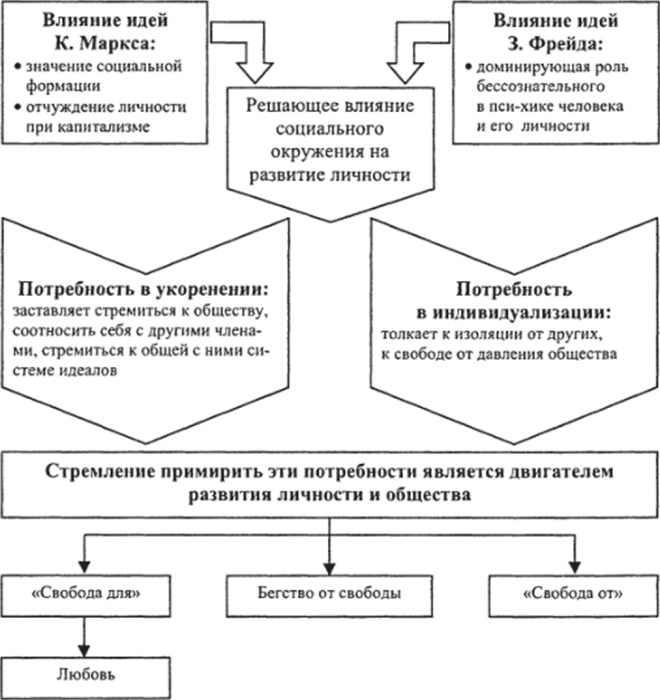
\includegraphics[width=\textwidth]{erich_fromm}

\end{flushleft}

\subsection{Список литературы}

\subsubsection{Рекомендумая литература}

\begin{enumerate}
    \item Васильев В.В., Кротов А.А., Бугай Д.В. История философии. М.: Академический проспект, 2008
\end{enumerate}

\subsubsection{Дополнительная литература}

\begin{enumerate}
    \item Гуревич П.С. Психоанализ. Т. 1. Фрейдизм и неофрейдизм. М.: Издательство Юрайт, 2019
\end{enumerate}

\section{Философия - 22.12.2022}

\subsection{Возникновение сознания и его социальная природа. Сознание и мозг}

\subsection{Сознание и язык. Виды и функции языка}

\begin{flushleft}

\textbf{Сущность языка} выявляется в его двуединой функции: служить средством общения и орудием мышления. \textbf{Речь} — это деятельность, сам процесс общения, обмена мыслями, чувствами, пожеланиями, целеполаганиями и т.п., который осуществляется с помощью языка, т.е. определенной системы средств общения.

\textbf{Язык} — это система содержательных, значимых форм. Язык выполняет роль механизма \textbf{социальной наследственности}.

Сознание и язык образуют \textbf{единство}: в своем существовании они предполагают друг друга, как внутреннее, логически оформленное идеально содержание предполагает свою внешнюю материальную форму. Язык есть \textbf{непосредственная деятельность мысли, сознания}. Он учавствует в процессе мыслительной деятельности как ее чувственная основа или орудие. Сознание не только выявляется, но и \textbf{формируется} с помощью языка. Мысли \textbf{строятся в соответствии с языком} и должны ему соответствовать. Справедливо и обратное: \textbf{мы организуем нашу речь в соответствии с логикой нашей мысли}.

Посредством языка происходит \textbf{переход от восприятий и представлений} к понятиям, протекает процесс оперирования понятиями. В речи человек фиксирует свои мысли, чувства и благодаря этому имеет \textbf{возможность подвергать их анализу} как вне его лежащий объект. Язык и сознание \textbf{едины}. В этом единстве определяющей стороной является сознание: будучи отражением действительности, оно «лепит» формы и диктует законы своего языкового бытия. Но единство — не тождество: сознание \textbf{отражает} действительность, а язык \textbf{обозначает} ее.

Язык и сознание образуют \textbf{противоречивое единство}. Язык влияет на сознание: его исторически сложившиеся нормы, специфичные у каждого народа, в одном и том же объекте оттеняют различные признаки. Однако зависимость мышления от языка \textbf{не является абсолютной}: мышление детерминируется главным образом своими связями с действительностью, язык же может лишь \textbf{частично модифицировать форму и стиль мышления}.

\end{flushleft}

\subsection{Сознание и самосознание}

\subsubsection{Теория о первичности сознания себя}

\begin{flushleft}

По \textbf{В.М. Бехтереву} (Владимир Михайлович Бехтерев), простейшей формой сознания следует признавать то состояние, когда еще не выработано ни одного более или менее ясного представления и суещствует лишь \textbf{неясное безотносительное чувствование собственного существования}.

Более сложным является сознание, в котором уже присутствуют те или иные представления. Но и в этом случае \textbf{наиболее элементарной формой} сознания следует признавать ту, при которой в сознании присутствует \textbf{главным образом одна группа представлений} о «Я» как субъекте в отличие от «не—Я» или объекта и из которой вырабатывается так называемое самосознание.

Лишь после этого возникают те формы сознания, которые основываются на пространственных и временных представлениях, и, наконец, как синтез первичного предметного созанния — формы, которые составляют «интимное ядро личности» и при которых человек \textbf{может анализировать} происходящие в нем самом психические процессы.

Для этой точки зрения характерно утверждение, что познание ребенком самого себя на первых этапах развития протекает \textbf{в отрыве от познания им окружающего мира} и даже в \textbf{отрыве от собственной деятельности}. Оно поддерживается исключительно за счет тех органических ощущений и чувствований, которые \textbf{даны ребенку от рождения}. Эти ощущения и чувства, таким образом перестают быть предпосылками в развитии самосознания и становятся \textbf{его источником и движущей силой}.

\end{flushleft}

\subsubsection{Теория об единстве развития сознания и самосознания}

\subsection{Список литературы}

\subsubsection{Рекомендуемая литература}

\begin{enumerate}
    \item Алексеев П.В., Панин А.В. Философия. М.: Издательство Проспект, 2005
    \item Спиркин А.Г. Философия: учебник. М. Гардарики, 2006
\end{enumerate}

\pagebreak
\section{Философия - 22.12.2022}

\subsection{Философия сознания}

\subsubsection{Историческая справка}

\begin{flushleft}

Уже в Древней Греции поднимались проблемы души (сознания) — \textbf{субстанциальное понимание} — как особого рода субстанции, строго отделенные от тела.

Сознание и тело онтологически отделены — \textbf{два разного рода субстанции}.

С появлением христианства \textbf{понимание о субстанциальное душе остается} — наследие древнегреческой мысли. Прожило до восьмидесятых годов двадцатого века.

Семнадцатый век — Декарт — базовые установки в теме сознания (мышления): cogito ergo sum, «центр мышления» — \textbf{мышление локализовано}, «шишковидная железа» — \textbf{хранилище души}.

Иммануил Кант — \textbf{трансцендентальный субъект} — центр познания.

\subsubsection{Современное положение}

Нейробиология положила конец картезианскому мифу о локализованном сознании.

Дэниел Деннет (основатель \textbf{функционализма}) — развенчал представление о «картезианский театр» — неправда, зрителя нет. У мозга есть \textbf{функции}; следует изучать сознание как набор функций.

\hfill

Аналитическая философия — \textbf{атлантическая школа}, тесная связь с нейронауками — философия сознания. Также есть континентальная школа. Некоторые буддистсткие школы заявляли об \textbf{отсутствии сознания}.

Дэвид Чалмерс — \textbf{легкие} (может быть решена эмпирически) и \textbf{трудные} (нерешаемая эмпирическими средствами) проблемы сознания: «каков характер связи между состояниями мозга и состояниями сознания?»

Есть несколько подходов к решению данной проблемы:

\begin{enumerate}
    \item Ее отмена — например, буддисты, исследователи-материалисты
    \item Непризнание ее сложной проблемой
    \item Попытки разложения ее на простые проблемы
\end{enumerate}

\paragraph{Вопрос о необходимости сознания} Зачем необходимо сознание? Миллионы биологических видов прекрасно живут без него. Концептуально это неясно.

\paragraph{Космологический подход} \textbf{Сильный антропологический принцип} — сознание \textbf{появилось по необходимости}, материя обладает потенцией к сознанию — потенция рано или поздно реализовывается.

\textbf{Слабый антропологический принцип} — появление мышления строго случайно.

\paragraph{Великая иллюзия сознания} Мы своего рода лишь \textbf{наблюдатели} собственной жизни — не непосредственные участники — \textbf{феноменальное сознание} (сознание ощущений) — очень малая часть того, что воспринимает мозг.

Мы не контролируем большую часть своей жизни — поддержание равновесия, пищеварение и так далее.

\paragraph{Проблема исследования сознания} Исследование сознания \textbf{ин-витро невозможно}, лишь \textbf{ин-виво} — методом интроспекции и самоотчета, что \textbf{необъективно}.

Мы можем делать выводы о сознании лишь исходя из степени правдоподобия.

\end{flushleft}

\end{document}